\section{Madness and the Primordial State}

\begin{wrapfigure}{rt}{.3\textwidth}
 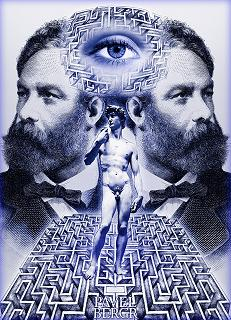
\includegraphics[scale=.5]{a20110131MadnessandthePrimordialState-img001.jpg} 
\end{wrapfigure}

Around 25 years or so ago, I attended a lecture by a Russian theosophist, then living in France. He described the spiritual experiences of an unusual young woman about 20 years of age. Coincidentally, on the way home, I was listening to a talk show on the radio, during which a young woman was describing her struggle with schizophrenia which began when she was also around 20 years old. I remember being struck by the similarity of the experiences of the two women. Unfortunately, I didn't take notes of either event, so I am unable to provide details. Nevertheless, the idea that mystical experience and schizophrenia are either similar or more likely often confused has stayed with me.

\paragraph{The Chiefest Blessings}
\textbf{Socrates} in the \emph{Phaedrus} distinguishes between madness as an evil or human infirmity and different kind of madness ``which is a divine gift, and the source of the chiefest blessings granted to men." As for the latter, they can be categorized as follows (with their respective sources of inspiration):

\begin{itemize}
\item \textbf{Prophetic} madness (Apollo) 
\item \textbf{Initiatory} madness (Dionysus) 
\item \textbf{Poetic} madness (Muses) 
\item \textbf{Erotic} madness (Aphrodite and Eros) 
\end{itemize}
Clearly, it would appear that at that time, there were many more men and women who were aware of a state closer to the Primordial State. They had a direct intuitive contact with the gods, which were the sources of the inspiration which, Socrates described, was ``a divine release of the soul form the yoke of custom and convention." Thus we see he is describing a state deeper than soul life. It is interesting to note, in passing, the structural similarity underlying the phenomena of prophecy, initiation, creativity, and love.

\paragraph{Schizophrenia}
In his work on the consciousness of men of early civilizations, \textbf{Julian Jaynes} makes note of the similarity of certain states of consciousness to schizophrenia. Although his perspective is scientistic, some of his observations are of value. He rightly points out that we sometimes accidentally slip into something resembling the Primordial State. For example, we may ``hear" critical voices, usually called the superego in psychology, or lose the sense of self, meaning the sense of the false self or analog I.

In the schizophrenic, these experiences are more extreme. Auditory hallucinations are stronger and their commands more insistent, there is the loss of the sense of ego, as well as his internalized mental model of the world. On the more positive side, the schizophrenic often demonstrates tirelessness, concentration, and sharper sensory perception.

Nevertheless, this is far from the \textbf{Primordial State}, given the dysfunction of the schizophrenic. Like other modern men, the schizophrenic is centered in the soul life. Thus, commands allegedly from the gods or other higher powers, are experienced as exterior to himself. Since his soul life is disordered, they are distorted by the turbulences in his own consciousness. He has no spirit, or \emph{nous}, to moderate his erotic and thumotic impulses, so the commands get confused and intermingled with unintelligent desires. This is why his behavior will be erratic, unpredictable, or even evil.

\paragraph{Metaphysical Interpretation}
The ``gods" represent higher non-formal states of being. Since in the Primordial State, one's center is in non-formal manifestation, the commands are not experienced as alien, but rather as originating from one's deepest center. To be experienced, however, they must be reflected in consciousness, that is, in one's soul life, or as subtle manifestation. In the Primordial State, that consciousness is pure and not disturbed by idle fantasies, random thoughts, negative emotions, pointless desires. Thus the commands are clear and unambiguous; hence they are the expression of one's True Will.

The center of the True Man transcends the soul life, which is experienced as exterior to himself, just as much so as is the exterior world of the trees, birds, mountains, and oceans.



\flrightit{Posted on 2011-01-31 by Cologero }

\begin{center}* * *\end{center}

\begin{footnotesize}\begin{sffamily}



\texttt{Exú on 2015-11-07 at 18:04 said: }

I can really tell about this subject,being my self a psychotic,not a schizoprenic but a paranoid,that means,a organized psychotic,i can really tell that i was always aware in a way or another,of the primordial self,that self that did not have any specific desire,or should i say,had the desire of cleaning my self from the pain,that was always exposed to me,since contrary to what happens to the neurotic,we do not have the repression that you"normal"people have,so the emotional pain was always following me,but it was not strong enought,to cloud the true self.The"unconciousness"is open to the psychotic,and we are geting more and more conscious.

\end{sffamily}\end{footnotesize}

